\chapter{Experimental Work}
\label{chap:experimental_work}

To test the data-driven controller in a real life experiment, a model-scale bicycle was chosen. The self-balancing mini-bike developed by \textbf{WHEELTEC} was utilized as the experimental platform. The primary goal of the project is to implement the data-driven controllers for stabilizing the bike. The mini-bike is equipped with various sensors and actuators to enable control and data acquisition.
\todo[inline]{Add Tapken's work on the same bike with simulink modelling for it. No: in intro better}
%% Mini-Bike Overview Section for Thesis

\section{Mini-Bike}
The mini-bike is based on the \textbf{WHEELTEC Z100 Servo Self-Balancing Bicycle} in Figure \ref{fig:minibike}. It features an STM32F103C8T6 microcontroller as the primary control unit, which integrates different sensors and motor control circuits to achieve stabilization.

\begin{figure}[htbp]
	\centering
	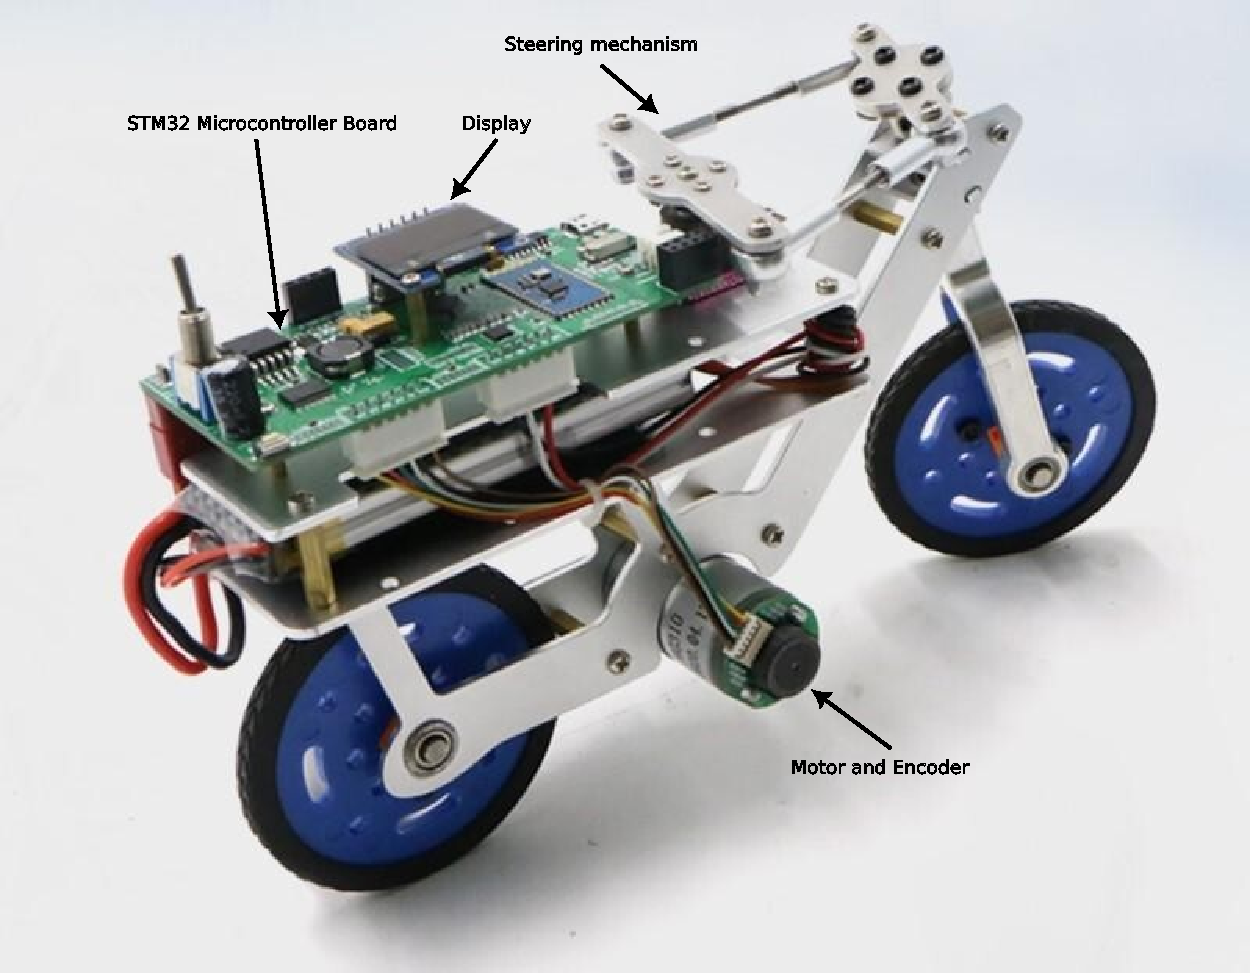
\includegraphics[width=0.7\linewidth]{figures/minibike/minibike_annotated.pdf}
	\caption{A picture for the MiniBike used in the experiments.}
	\label{fig:minibike}
\end{figure}

%\subsection{Mini-Bike Structure and Components}


The bike has the following key components:
\begin{itemize}
	\item \textbf{Microcontroller:} STM32F103C8T6 (ARM Cortex-M3)
	\item \textbf{IMU Sensor:} MPU6050 (3-axis gyroscope and accelerometer)
	\item \textbf{Servo Motor:} WHEELTEC Z100 steering servo
	\item \textbf{Rear Wheel Motor:} DC motor with incremental encoder
	\item \textbf{Motor Driver:} AT8236 H-bridge circuit
	\item \textbf{Power Supply:} 2S lithium-ion battery (7--12 V)
	\item \textbf{Wireless Communication:} Bluetooth module (USART3)
\end{itemize}

%\subsection{Balancing and Control Mechanism}

The bike uses steering angle control to self-balance. This is done through an LQR followed by a PID controller. The LQR computes the state-feedback gain that minimises the cost function. While the PID controller adjusts the PWM signals to the servo motor to fine-tune the steering speed.

The bike is balanced continuously through getting data from the gyroscope, which provides real-time data on tilt angles and angular velocities. The microcontroller operated at a frequency of 100 Hz. The measurements are processed by the microcontroller to compute the control law, where the input is the steering angle derivative.

The Data was collected from the bike through a Bluetooth connection using USART3, where the frequency of data was about 10 Hz. A mobile device was connected to the bike where the data received was saved for processing.

The mini-bike allows adjustment of the balance midpoint through a potentiometer; if it is offset from zero, the bike will move in a circle in the direction of the lean. Moving in a circle allowed for a longer range of data collected while driving under a controller.

The control algorithms were implemented on the STM32 using C++ programming with HAL Drivers.
The platform on which the development of codes were done is the \textit{stm32cube programmer}, which is a free unlimited software for writing and building the codes. It compiled the codes into a Hexadecimal file which can then be flashed on the STM32 microcontroller using FlyMCU software.

The codes read the IMU data (lean angle and angular velocity) via I2C communication. Then, the forward velocity is estimated by processing the encoder pulses. The lean angle is estimated by a complementary filter. The implemented control law is then applied using the states and a control input is determined. Consequently, the PWM signal of the steering servo is computed and applied.

The data-driven MPC controller was not implemented since the real-life errors prevented successful solving of the SDP on real data as stated before. Due to this limitation, the SDP optimisation was first performed offline, and the resulting state-feedback gain matrix was embedded into the embedded controller as a static gain.

The system states that were recorded are the lean angle ($\phi$), lean rate ($\dot{\phi}$), and Steering angle ($\delta$).

\section{Experiments}
Four different controllers were applied on the mini-bike based on both the LQR and data-driven state-feedback discussed in \autoref{chap:simulations}. The experiments are described in \autoref{tab:controllers_summary}.

\begin{table}[H]
	\centering
	\caption{Overview of controllers applied on the mini-bike}
	\label{tab:controllers_summary}
	\begin{tabular}{|c|c|c|c|}
		\hline
		\textbf{Experiment} & \textbf{Controller} & \textbf{Target Angle}  & \textbf{Target Angle} \\ \hline
		1 & LQR & $75^\circ$  & $4^\circ$ \\ \hline
		2 & LQR & $90^\circ$  &  $5^\circ$ \\ \hline
		3 & Data-driven state-feedback & $75^\circ$  &  $3.5^\circ$ \\ \hline
		4 & Data-driven state-feedback & $90^\circ$  &  $4^\circ$ \\ \hline
	\end{tabular}
\end{table}

The results acquired on implementing the controllers and collecting the data are plotted in \autoref{fig:experiments}. It can be noticed that the data length varies across the 4 experiments. This is due to the capability of collecting the data before the bicycle falls, particularly in experiment 3 in \autoref{fig:exp3}, where the controller did not maintain bicycle balance for an extended period.

\begin{figure}[htbp]
	\centering
	\begin{subfigure}[b]{\textwidth}
		\centering
		
\includegraphics[width=\textwidth]{figures/experiments_plots/line_plot_Exp_1_fast_data_target_4.0_degrees_Fixed_screw_avg_4.36.pdf}
		\caption{\boldmath LQR for $75^\circ$ fork angle and $4^\circ$ target angle.}
				\label{fig:exp1}
	\end{subfigure}
	\vspace{0.5cm}
	\begin{subfigure}[b]{\textwidth}
		\centering
		
\includegraphics[width=\textwidth]{figures/experiments_plots/line_plot_Exp_2_fast_data_target_5_degrees_avg_5.99.pdf}
		\caption{\boldmath LQR for $90^\circ$ fork angle and $5^\circ$ target angle.}
				\label{fig:exp2}
	\end{subfigure}
\end{figure}
%	\vspace{0.5cm}
\begin{figure}[htbp]\ContinuedFloat
	\centering
	\begin{subfigure}[b]{\textwidth}
		\centering
		
\includegraphics[width=\textwidth]{figures/experiments_plots/line_plot_Exp_3_fast_data_target_3.5_degrees_Fixed_screw_avg_5.21.pdf}
		\caption{\boldmath Data-driven state-feedback for $75^\circ$ fork angle and $3.5^\circ$ target angle.}
				\label{fig:exp3}
	\end{subfigure}
	\vspace{0.5cm}
	\begin{subfigure}[b]{\textwidth}
		\centering
		
\includegraphics[width=\textwidth]{figures/experiments_plots/line_plot_Exp_4_fast_data_target_4.0_degrees_Fixed_screw_avg_4.24.pdf}
		\caption{\boldmath Data-driven state-feedback for $75^\circ$ fork angle and $4^\circ$ target angle.}
				\label{fig:exp4}
	\end{subfigure}
	\caption{\boldmath Lean angle over time under different data-driven state-feedback settings for an initial state vector (in radians) $x_0 = [0.0873, \, 0, \, 0]^\top$, $Q = \operatorname{diag}(300,\,0.1,\,300)$, $R = 1$, noise bound $\epsilon = 0.001$ and data length of $T = 40$.}
	\label{fig:experiments}
\end{figure}
